\documentclass[a4paper, 12pt]{extarticle}

% Import packages
%------------------------------------------------
\usepackage{csquotes}        % for Russian quotes
\usepackage[utf8]{inputenc}  % utf8 encoding
\usepackage[russian]{babel}  % enable Russian language
\usepackage{titling}         % for \thetitle, \thedate
\usepackage{enumitem}        % for lists customization
\usepackage{graphicx}        % for adding images
\usepackage{prettyref}       % for configuring references
\usepackage{caption}         % for figure caption customization
\usepackage{subcaption}      % for \subfigure
%------------------------------------------------

% Geometry
%------------------------------------------------
\usepackage{geometry}
\geometry{
    top=1.5cm,        % Top margin
    bottom=1.5cm,     % Bottom margin
    left=2cm,         % Left margin
    right=2cm,        % Right margin
    includefoot,      % Include space for a footer
}
%------------------------------------------------

% Table of Context
%------------------------------------------------
\usepackage[titles]{tocloft} % style of table of context
\usepackage{hyperref}        % clickable table of context items

\setcounter{tocdepth}{2}     % set ToC depth. (2: sections+subsubsections)

\renewcommand{\cftsecafterpnum}{\vspace{10pt}}    % set space after section
\renewcommand{\cftsubsecafterpnum}{\vspace{5pt}}  % set space after subsection

\renewcommand{\cftsecfont}{\bfseries \large}      % change section font

\hypersetup{
    colorlinks,
    citecolor=black,
    filecolor=black,
    linkcolor=black,
    urlcolor=black
}
%------------------------------------------------

% Sections style
%------------------------------------------------
\usepackage{titlesec} % for changing style of sections

% Section settings
\titleformat{\section}
{\bfseries\LARGE}
{\thesection. }
{4pt}
{}
[{\titlerule[0.4pt]}]

% Subsection settings
\titleformat{\subsection}
{\bfseries\Large}
{\thesubsection. }
{0pt}
{}

% Subsubsection settings
\titleformat{\subsubsection}
{\bfseries\large}
{}
{0pt}
{}
%------------------------------------------------

% Other settings
%------------------------------------------------
\setlength{\parindent}{0pt}
\setlist{itemsep=1pt}
\newrefformat{fig}{(рис. \ref{#1})}
%------------------------------------------------

% Title, author, date
%------------------------------------------------
\title{Анализ распространения COVID-19 в России}
\author{Якубов Камиль и Меркулов Вадим}
\selectlanguage{russian}
\date{\today}
%------------------------------------------------

\begin{document}
\begin{titlepage}
    \vspace*{5cm}
    \begin{center}

        \huge{\textbf{\thetitle}}

        \vspace{2 cm}
        \large
        Подготовили:\\
        \Large{\theauthor}
        \vfill
        \large
        \thedate

    \end{center}
\end{titlepage}

\tableofcontents
\newpage

\section{Введение}

В 2020 году люди почти всех стран мира перенесли на себе последствия карантина
и массового локдауна, связанного со стремительными темпами распространения
инфекции, вызванной новым коронавирусом SARS-CoV-2. Исследования этого
заболевания ведутся во всех ведущих странах мира, наука всеми силами стремится
ускорить процесс изучения вируса для эффективной борьбы с ним. Анализ данных,
собранных о коронавирусе как никогда необходим и важен как для научных
деятелей, так и для простых граждан, ведь, исследовав уже имеющиеся данные,
стало возможным предотвращение множества новых случаев заболевания.
\\

Темой нашего проекта является темп распространения COVID-19 в Российской Федерации. Актуальность исследования связана со стремительным ростом числа заболевших данной инфекцией в нашей стране, а также с незнанием реальной опасности коронавируса на фоне второй волны эпидемии.
\\

Мы постараемся ответить на вопрос: \textquote{Как распространялась
коронавирусная инфекция COVID-19 в Российской Федерации?}
\\

 Целью данной работы является наглядное изучение особенностей распространения вируса в России с помощью графиков и диаграмм.
\\

\begin{normalsize}
    \textbf{Задачи:}
\end{normalsize}
\begin{itemize}
    \item[\bfseries--] проанализировать темпы распространения коронавируса в России;
    \item[\bfseries--] сравнить показатели первой и второй волны коронавирусной инфекции в России;
    \item[\bfseries--] узнать, какие регионы Российской Федерации пострадали в большей степени;
    \item[\bfseries--] выяснить, были ли предпринятые властями меры эффективными.
\end{itemize}

В связи с этим, предметом исследования станет инфекция
COVID-19, а объектом — ее распространение на территории нашей страны.
\newpage

\section{Основные сведения о COVID-19}
\subsection{История появления и распространения вируса}

В декабре 2019 года новый коронавирус неизвестного происхождения был
идентифицирован у нескольких пациентов в городе Ухань провинции Хубэй в Китае.
Большая часть первых заболевших имела отношение к местному рынку, на котором
продаются морепродукты, а также птицы, змеи, летучие мыши и
сельскохозяйственные животные.
\\

В ходе расшифровки генома коронавируса в нём были обнаружены составные части, близкие коронавирусам летучих мышей и
панголинов. Считается, что на территории Уханьского рынка произошла встреча
летучих мышей и панголинов, создавшая условия для рекомбинации коронавирусов
этих животных. Однако согласно муниципальным отчётам, летучие мыши никогда не
продавались на местном рынке, а панголины занесены в Красную книгу.
\\

Китай сообщил о своей первой смерти, связанной с COVID-19, 11 января, а 13
января был выявлен первый случай заболевания за пределами Китая. В феврале 2020
года инфекция начала быстро распространяться по разным странам, несмотря на
принимаемые властями Китая карантинные меры. В то же время, в самом Китае со
вспышкой инфекции ко второй половине марта удалось в основном справиться. 19-20
марта в континентальном Китае не было зарегистрировано новых случаев заражения
(хотя и были выявлены инфицированные, прибывшие из-за рубежа).
\\

Первый случай за пределами Китая стал известен 13 января. Это была 61-летняя
женщина, которая прилетела из Уханя 8 января в Бангкок (Таиланд). К 18 января
количество случаев за пределами Китая увеличилось до трёх случаев (два в
Таиланде, один в Японии).
\\

20 января китайские власти сообщили о резком увеличении числа новых случаев
заболевания, вызванного коронавирусной инфекцией COVID-19, сразу на 140 новых
пациентов; некоторые из них оказались за пределами Уханя — в Шэньчжэне и
Пекине. Также сообщалось о ещё одной смерти, вызванной вирусом, и о первом
случае заболевания в Южной Корее. Китайские власти официально подтвердили, что
имели место случаи передачи инфекции от человека к человеку.
\\

30 января ВОЗ объявила эпидемию чрезвычайной ситуацией в области общественного
здравоохранения, имеющей международное значение, а 11 февраля болезнь,
вызванная вирусом, получила свое официальное название — COVID-19. По состоянию
на 13 декабря 2020 года, в ходе пандемии было зарегистрировано свыше 72 млн
случаев заболевания по всему миру; более  1,613 млн человек скончалось и более
50,6 млн выздоровело.
\\

Первые случаи заболевания COVID-19 на территории России были зарегистрированы
31 января 2020 года: один в Тюмени, а другой — в Чите. Оба заболевших были
гражданами Китая.
\newpage

\subsection{Симптомы и осложнения заболевания}
\vspace{3mm}

\textbf{Часто наблюдаемые симптомы:}
\begin{itemize}
    \item повышение температуры тела;
    \item сухой кашель;
    \item утомляемость.
\end{itemize}

\vspace{5mm}

\textbf{У некоторых инфицированных могут также наблюдаться:}
\begin{itemize}
    \item различные болевые ощущения;
    \item боль в горле;
    \item диарея;
    \item конъюнктивит;
    \item головная боль;
    \item потеря обоняния и вкусовых ощущений;
    \item сыпь на коже или депигментация ногтей на руках и ногах.
\end{itemize}

\vspace{5mm}

\textbf{Симптомы тяжелой формы заболевания:}
\begin{itemize}
    \item затрудненное дыхание или одышка;
    \item ощущение сдавленности или боль в грудной клетке;
    \item нарушение речи или двигательных функций.
\end{itemize}

\vspace{5mm}

\textbf{Необходимо знать:}
\begin{itemize}
    \item[\bfseries--] Вирус передается воздушно-капельным путем и при непосредственном
        контакте людей. Вирус не передается через воду или при плавании;
    \item[\bfseries--] Возбудителем COVID-19 является вирус из семейства коронавирусов.
        Антибиотики на вирусы не действуют;
    \item[\bfseries--] Если у вас наблюдаются симптомы тяжелой формы заболевания,
        незамедлительно обратитесь за медицинской помощью. Прежде чем посещать
        клинику или больницу, позвоните и предупредите о своем визите;
    \item[\bfseries--] Людям, у которых наблюдаются умеренно выраженные симптомы и нет
        других заболеваний, рекомендуется симптоматическое лечение в домашних
        условиях;
    \item[\bfseries--] В среднем между моментом инфицирования и появлением симптомов
        проходит 5–6 дней, однако в некоторых случаях этот период может
        занимать до 14 дней.
\end{itemize}
\newpage

\subsection{Социально-экономические последствия пандемии}
\subsubsection{Финансы}

Распространение коронавируса привело к глобальному обвалу фондового рынка,
который начался 20 февраля 2020 года. Множество крупных промышленные индексов
упало 27 февраля в одну из худших торговых недель после финансового кризиса
2007—2008 годов. 9 марта индексы Уолл-стрит упали более на 7\%. Падение
получило название Чёрный понедельник и было худшим падением со времён Великой
рецессии в 2008 году. Через три дня после Чёрного понедельника произошло ещё
одно падение — Чёрный четверг, когда акции по всей Европе и Северной Америке
упали более на 9\%. На Уолл-стрит произошло самое большое однодневное снижение
процентных ставок со времён Чёрного понедельника в 1987 году, а индекс FTSE
Mors of Borsa Italiana упал более на 17\%, став самым пострадавшим рынком во время Чёрного четверга.

\subsubsection{Экономика}

Непосредственно пандемия привела к закрытию предприятий в странах с высоким
процентом заболевших, резкому возрастанию спроса на продукты повседневного
спроса, спекуляциям на рынке определённых товаров: противовирусных препаратов,
санитарных масок, дезинфицирующих средств.
\\

Пандемия привела к значительному росту спроса на услуги доставки еды из-за
нежелания (в некоторых странах и регионах — запрета) многих граждан выходить из
дома. При этом стали возникать опасения того, что заражение коронавирусом может
распространяться через курьеров. Ответом на эти опасения стала бесконтактная
доставка продуктов питания и других товаров.
\\

Из-за остановки предприятий в Китае, а затем и во всём мире спрос на нефть и
нефтепродукты значительно упал. На фоне снижения спроса Россия и ОПЕК не смогли
договориться о сокращении добычи нефти и начали ценовую войну на рынке
углеводородов что, в свою очередь, привело к обрушению цен на нефть.
\\

Продолжительный карантин изменил приоритеты потребления: упал спрос на ряд
товаров, такие как автомобили и одежда, но при этом вырос спрос на товары для
дома, как на облегчающие домашний быт, так и на домашний спорт и на развлечения
(онлайн-игры, стриминговые сервисы). Также вырос спрос на товары для домашнего
офиса, так как многие виды работ стали удалёнными, и соответственно переживают
пик популярности приложения для видеоконференций такие как Zoom, Microsoft
Teams и их аналоги.

\subsubsection{Культура}
По всему миру в той или иной степени было ограничено посещение кинотеатров,
кинофестивали были отменены или отложены, кинорелизы передвинуты на будущие
даты, кинопроизводство приостановлено.
\\

Однако вместе с тем потоковое вещание стало более популярным. В связи с этим
таким крупным стриминговым сервисам, как Netflix и YouTube, пришлось снизить качество потокового видео чтобы
снизить нагрузку на провайдеров).
\\

Было отменено или отложено множество фестивалей, выставок и конкурсов, включая
Московский международный кинофестиваль, Каннский кинофестиваль, и конкурс песни
«Евровидение-2020».
\\

Из-за пандемии театры, музеи, художественные галереи и другие культурные
учреждения по всему миру оказались закрыты. Объёмы оказываемой им финансовой
поддержки сильно зависят от страны, если в США было выделено 200 миллионов
долларов в качестве помощи культурным институциям, то Германия выделила 50
миллиардов евро, а власти Испании заявили, что на время пандемии культура
должна стоять на последнем месте в списке приоритетов.
\newpage

\subsection{Вывод}
После анализа всех имеющихся данных можно сделать вывод, что
при поражении коронавирусной инфекцией человек может столкнуться с большим числом
осложнений: страдают как легкие, так и почки, кишечник, нервная система. Так же
подобное состояние в купе с массовыми заражениями по всему миру могут негативно
влиять и на психическое состояние больного.
\\

После непосредственного попадания инфекции в организм человека могут появиться
различные симптомы: повышенная температура, слабость, ломота в теле, першение в горле.
Все очень похоже на достаточно известное заболевание - ОРВИ. Кажется, что нет
оснований для беспокойства. И вдруг состояние резко ухудшается - возникает
выраженная одышка, ощущение нехватки воздуха. При появлении похожих признаков
необходимо как можно скорее вызвать врача на дом.
\\

Факторы, затрудняющие выздоровление:
\begin{itemize}
    \item[\bfseries--] Ожирение;
    \item[\bfseries--] Сахарный диабет;
    \item[\bfseries--] Сердечно-сосудистые заболевания
    \item[\bfseries--] Пожилой возраст;
\end{itemize}

Поэтому в особенности пожилым пациентам, тем, кто страдает от ожирения, и/или имеет
предрасположенность к сердечно-сосудистыми заболеваниями необходимо быть
особенно бдительными и в случае заболевания и COVID-19 вовремя обращаться к
врачам.
\\

При новой коронавирусной инфекции существенно страдают легкие. На компьютерной
томографии диагностируются поражения легочной ткани, типичные для этого
заболевания. Но помимо этого новый коронавирус вызывает в организме
генерализованную воспалительную реакцию, у части пациентов чрезвычайно бурную,
так называемый цитокиновый шторм. При этом состоянии в крови пациентов
определяются очень высокие показатели цитокинов (интерлейкинов) - маркеров
воспаления, высвобождение которых предполагает причинение вреда собственным
клеткам организма. И это грозит развитием серьезных осложнений.
\\

На данный момент над борьбой с COVID-19 работают многие
страны мира, и налицо результаты их трудов. Однако, прошло слишком мало времени,
чтобы все страны мира были обеспечены новой вакциной, разработанной немецкими
учеными с пока еще рабочим названием \textquote{BNT162b2}, снижающей риск заболевания на
90\% согласно собранной статистике.
\\
\newpage

\section{Распространение коронавируса в России}
\subsection{Сбор данных}
\subsubsection{Сбор данных о подтвержденных случаях за сутки}

Для сбора информации о новых случаях заболевания на территории Российской
Федерации мы использовали данные с официального сайта Роспотребнадзора. Каждый
день Роспотребнадзор публикует статью во вкладке \textquote{Новости},
содержащую информационную сводку с числом заболевших новым коронавирусом по
регионам. Чтобы собрать эти данные, мы создали скрипт на языке Python, который
сохраняeт ссылки на новостные статьи в отдельном файле, а затем с помощью
модулей \textquote{requests} и \textquote{BeautifulSoup} из библиотеки Python
мы извлекаем статистику о заболевших из HTML разметки сайта. Полученные записи
сохраняем в двух электронных таблицах \textquote{csv}. В первой таблице хранятся
данные о новых зараженных по регионам, а во второй данные по всей России \prettyref{fig:collection1_res}.

\begin{figure}[h]
    \centering
    \begin{tabular}[c]{cc}
    \begin{subfigure}[b]{0.49\textwidth} \centering
        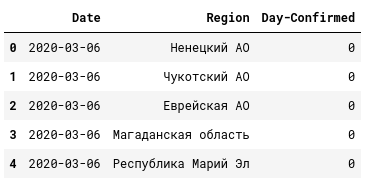
\includegraphics[height=130pt]{../plots/regions_df1.png}
        \caption{Данные по регионам} \label{fig:regions_df1}
    \end{subfigure}&

    \begin{subfigure}[b]{0.49\textwidth} \centering
        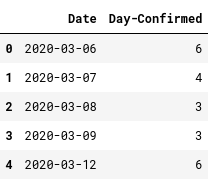
\includegraphics[height=130pt]{../plots/country_df1.png}
        \caption{Данные по России} \label{fig:country_df1}
    \end{subfigure}
    \end{tabular}
    \caption{Электронные таблицы} \label{fig:collection1_res}
\end{figure}

\subsubsection{Сбор данных о выздоровевших и умерших за сутки}

Для получения статистики о выздоровевших и умерших за сутки мы использовали
данные с официального сайта оперативного штаба \textquote{Стопкоронавирус.рф}.
Они так же, как и Роспотребнадзор, публикуют статьи с информацией о динамике
распространения коронавируса, а именно данные о выздоровевших и умерших за
сутки по регионам страны. По аналогии со сбором данных о подтвержденных случаях за сутки мы создали скрипты на языке \textquote{Python}, которые извлекают из HTML разметки сайта необходимую нам информацию. Однако мы заметили, что до 6 мая на сайте \textquote{Стопкоронавирус.рф} ежедневная статистика не имела единого шаблона, что затрудняло нашу работу. Поэтому мы решили заполнить пропущенные данные информацией из уже существующей базы данных по коронавирусу в России. Полученные значения мы объединили с данными о подтвержденных случаях. \prettyref{fig:collection2_res}

\begin{figure}[h]
    \centering
    \begin{tabular}[c]{cc}
    \begin{subfigure}[b]{\textwidth} \centering
        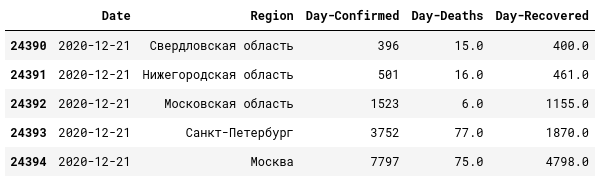
\includegraphics[height=130pt]{../plots/regions_df2.png}
        \caption{Данные по регионам} \label{fig:regions_df2}
    \end{subfigure}& \\

    \begin{subfigure}[b]{\textwidth} \centering
        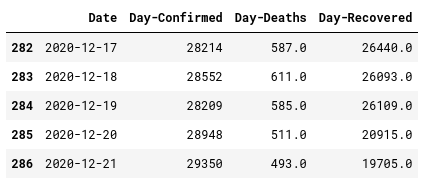
\includegraphics[height=130pt]{../plots/country_df2.png}
        \caption{Данные по России} \label{fig:country_df2}
    \end{subfigure}
    \end{tabular}
    \caption{Электронные таблицы} \label{fig:collection2_res}
\end{figure}
\newpage

\subsection{Связь России и Москвы}

Будучи как центром бизнеса, так и всей экономики Российской Федерации, Москва
стала ко всему прочему еще и одним из центров заражения коронавирусной
инфекцией всей страны. Столица по уровню заболеваемости COVID-19 вышла на пиковые
значения в середине весны.
\\

Резкий рост наблюдался в апреле 2020 года,
что впоследствии было названо первой волной коронавируса, ее легко распознать
на графике \prettyref{fig:day_confirmed_russia_moscow}. На этом временном отрезке можно видеть, что поведение
графика заражений во всей стране схоже с рисунком, который образует график
заражений в одной лишь Москве. Заметим, что разрыв (расстояние от пиков одного графика до
соответствующих пиков другого) между двумя этими графиками заметно меньше, чем
тот же разрыв, но уже в период второй волны заражения.
\\

Теперь наглядно можно видеть, что
в весенний период Москва являлась одним из формообразующих факторов ситуации с
коронавирусом в целой стране.
\\

\begin{figure}[h]
    \centering
    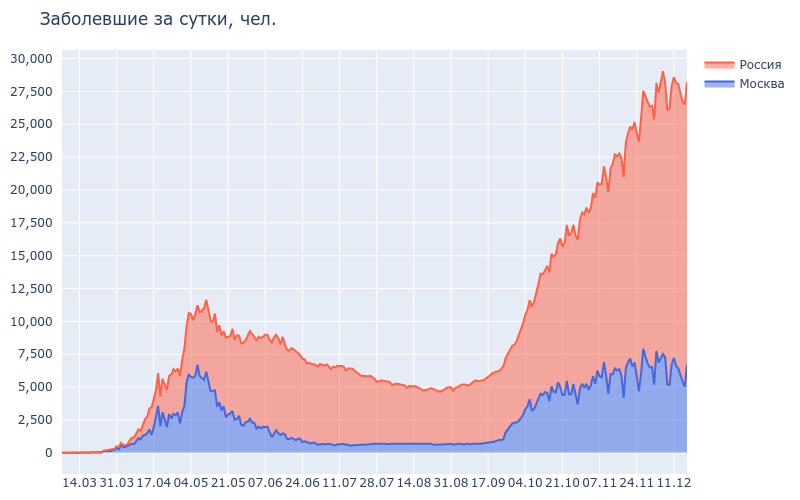
\includegraphics[scale=0.55]{../plots/1day_confirmed_russia_moscow.png}
    \caption{Заболевшие за сутки, чел.} \label{fig:day_confirmed_russia_moscow}
\end{figure}


\newpage

\phantomsection
\addcontentsline{toc}{section}{Список литературы}
\begin{thebibliography}{9}
\bibitem{latexcompanion}
Michel Goossens, Frank Mittelbach, and Alexander Samarin.
\textit{The \LaTeX\ Companion}.
Addison-Wesley, Reading, Massachusetts, 1993.
\end{thebibliography}


\end{document}
